\chapter{Eksperymenty}

\section{Pierwszy krok kaskady - lokalizacja frontu autobusu}

\subsection{Zbiór danych uczących i testowych}

Pierwszą partią danych ucząco-testowych było 11 zestawów obrazów
przygotowanych z~uprzednio pobranych filmów z~serwisu YouTube.

Każdy zestaw składał się z co najmniej dwuch zbiorów obrazów 
reprezentujących oznaczone fronty autobusów oraz obrazy tła
(ang. background). Opcjonalnym zbiorem był zestaw oznaczonych 
frontów autobusów typu solaris. Osobny zestaw frontów miał na celu
porównanie skuteczności detektorów przygotowanych tylko przy pomocy
pojedynczego typu obiektu oraz tych do przygotowania których użyto
obiektów znacząco od siebie różnych.

\newpage
\subsubsection{Zbiór jJ9ixBfVR5k}

W~zbiorze znalazły się następujące typy autobusów: 
\begin{itemize}
    \item Jelcz: M121M (x:3,y:1), M121CNG (x:4,y:1),
    \item Ikarus 280 (x:1, y:1),
    \item Man: NL223 (x:2, y:[1:2]), (x:3, y:2 - zielony wyświetlacz),
        Lion's City (x:4, y:2),
    \item Scania OmniCity CN (x:1, y:2). 
\end{itemize}
Współrzędne w~nawiasach określają pozycję modelu augobusu na rysunku
\ref{fig:jJ9ixBfVR5k_types}.
Jaden z modeli autobusów Man został wyposażony w zielony wyświetlacz numeru.
Jet to bardzo trudny przypadek w kontekście rozpoznawania numeru.

\begin{figure}[!h]
    \centering
    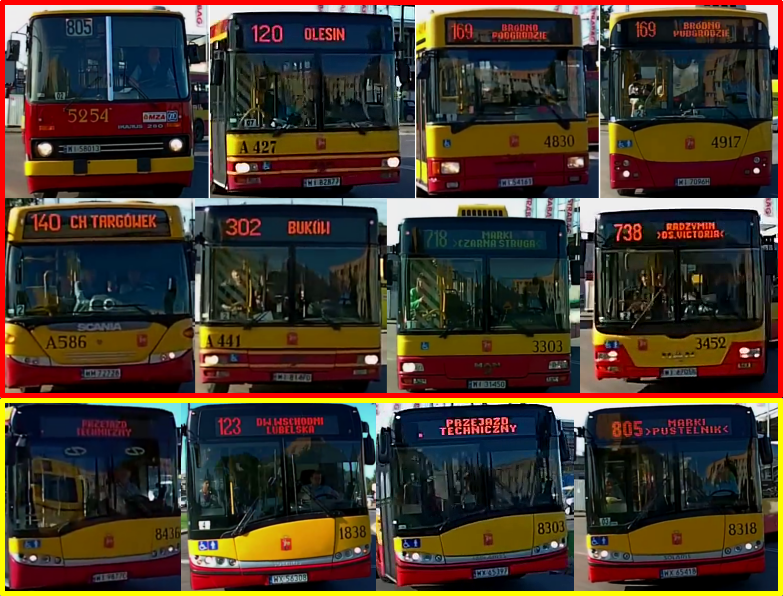
\includegraphics[width=0.9\textwidth]{img/exp_trainig_data_jJ9}
    \caption{Typy autobusów zawarte w zbiorze jJ9ixBfVR5k}
    \label{fig:jJ9ixBfVR5k_types}
\end{figure}

Liczebność zebranych próbek została przedstawiona w~tabelce nr. 
\ref{tab:jJ9ixBfVR5k_count}. Jest to jeden z~najliczniejszych zbiorów
przeznaczonych do uczenia i~testowania detektora kaskadowego w~tym 
opracowaniu.

\begin{table}[!h]
    \centering
    \begin{tabular}{c|c|c}
        Front   & Solaris   & Background \\
        2587    & 222       & 2239
    \end{tabular}
    \caption{Liczebność zbioru jJ9ixBfVR5k}
    \label{tab:jJ9ixBfVR5k_count}
\end{table}

\newpage

\subsubsection{Zbiór vYqZ4-tH4M0}

W~zbiorze znalazły się te same dwa modele autobusu Jelcz co w~zbiorze
poprzednim. Powtórzyły się także modele: Ikarus, Scania oraz dwa modele
autobusów Man. Dodatkowo pojawił się model: Mercedes Citaro, oraz trzy 
niezidentyfikowane bliżej modele - pozycje: druga, trzecia i~czwarta 
w~rzędzie drugim na rysunku \ref{fig:vYqZ4-tH4M0_types} 
(prawdopodobnie Solaris, Autosan oraz Jelcz).

\begin{figure}[!h]
    \centering
    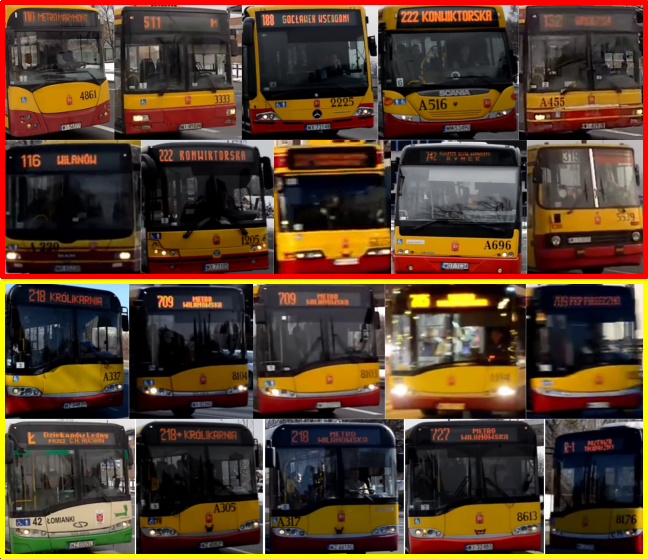
\includegraphics[width=0.9\textwidth]{img/exp_trainig_data_vYq}
    \caption{Typy autobusów zawarte w zbiorze vYqZ4-tH4M0}
    \label{fig:vYqZ4-tH4M0_types}
\end{figure}

Jeżeli chodzi o~liczebność to zbiór ten plasuje się w~środku stawki.
Dokładne dane zamieszczono w~tabeli \ref{tab:vYqZ4-tH4M0_count}.

\begin{table}[!h]
    \centering
    \begin{tabular}{c|c|c}
        Front   & Solaris   & Background \\
        291     & 320       & 230 
    \end{tabular}
    \caption{Liczebność zbioru vYqZ4-tH4M0}
    \label{tab:vYqZ4-tH4M0_count}
\end{table}

\newpage

\subsubsection{Zbiór J8h8j6096Uw}

W~zbiorze zabrakło zdjąć reprezentujących fronty autobusów marki
Solaris. Znalazły się natomiast dwa modele marki Man - wersja 
z~,,płaską'' maską (NL223) oraz model z~charakterystycznym czarnym
wgłębieniem w~centralnej jej części (Lion's City).

\begin{figure}[!h]
    \centering
    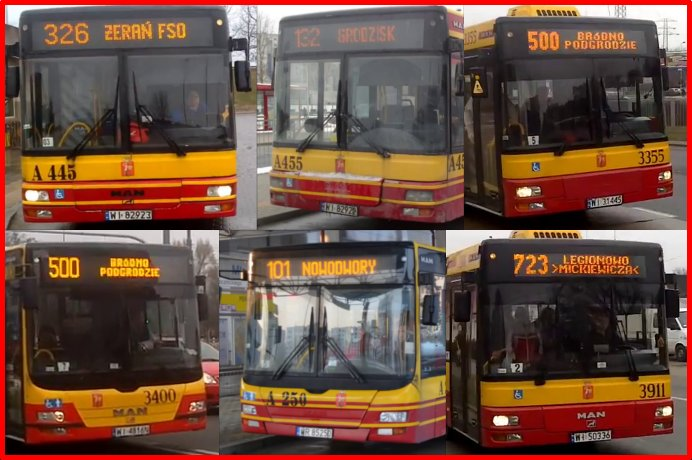
\includegraphics[width=0.65\textwidth]{img/exp_trainig_data_J8h}
    \caption{Typy autobusów zawarte w zbiorze J8h8j6096Uw}
    \label{fig:J8h8j6096Uw_types}
\end{figure}

\begin{table}[!h]
    \centering
    \begin{tabular}{c|c|c}
        Front   & Solaris   & Background \\
        182     & brak      & 427 
    \end{tabular}
    \caption{Liczebność zbioru J8h8j6096Uw}
    \label{tab:J8h8j6096Uw_count}
\end{table}

\subsubsection{Zbiór aO71uxrP9B0}

W~zbiorze miejsce znalazły zaledwie dwa modele autobusu Volvo plus 
występujący już wcześniej Mercedes Citaro.

\begin{figure}[!h]
    \centering
    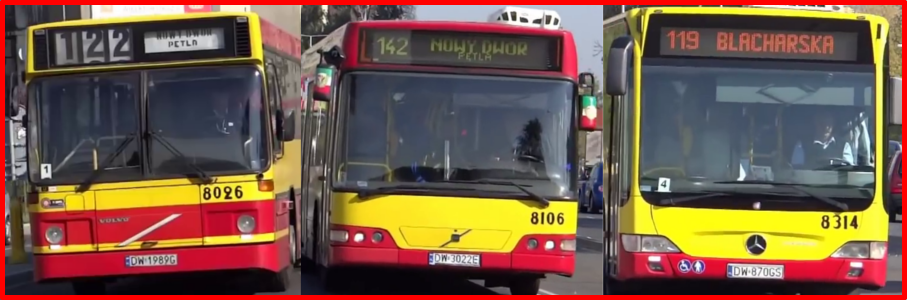
\includegraphics[width=0.65\textwidth]{img/exp_trainig_data_aO7}
    \caption{Typy autobusów zawarte w zbiorze aO71uxrP9B0}
    \label{fig:aO71uxrP9B0_types}
\end{figure}

\begin{table}[!h]
    \centering
    \begin{tabular}{c|c|c}
        Front   & Solaris   & Background \\
        177     & brak      & 977 
    \end{tabular}
    \caption{Liczebność zbioru aO71uxrP9B0}
    \label{tab:aO71uxrP9B0_count}
\end{table}

\newpage

\subsubsection{Zbiór J6sD0Tc2Dbs}

Zbiór ten zawiera dwa rodzaje autobusów marki Man oraz dwie wersje autobusu
Solaris - ze znaczkiem na masce oraz bez niego (maska gładka). Wyświetlacze
prezentujące numer wykorzystane w~przedstawionych modelach Solarisów
skutecznie uniemożłiwiają odczytanie go przez jakiekolwiek urządzenie. 
Nawet człowiek nie jest w~stanie domyślić się numeru który został utrwalony
na zdjęciach - rysunek \ref{fig:J6sD0Tc2Dbs_types}. Historyczne modele
skody zostały zaprezentowane w~ramach ciekawostki i~nie będą uwzględniane
w~dalszych eksperymentach.

\begin{figure}[!h]
    \centering
    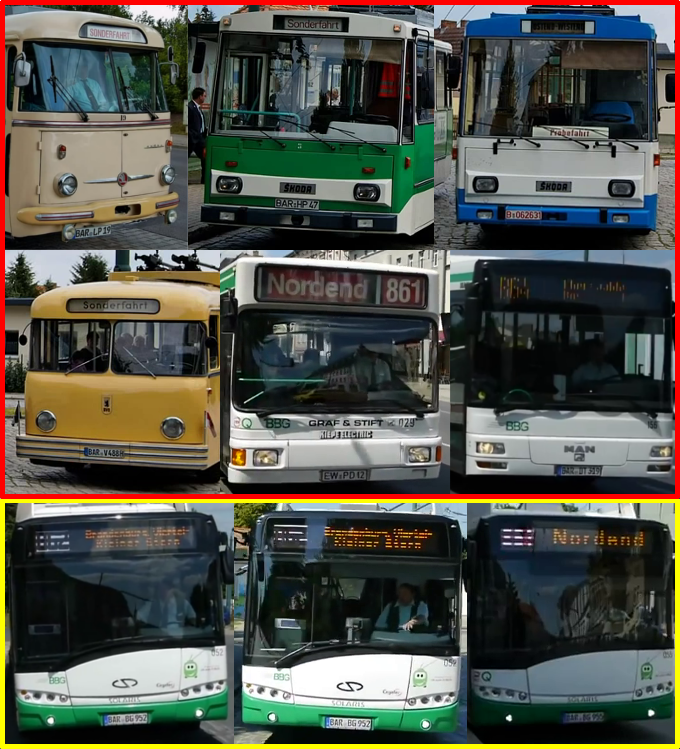
\includegraphics[width=0.65\textwidth]{img/exp_trainig_data_J6s}
    \caption{Typy autobusów zawarte w zbiorze J6sD0Tc2Dbs}
    \label{fig:J6sD0Tc2Dbs_types}
\end{figure}

\begin{table}[!h]
    \centering
    \begin{tabular}{c|c|c}
        Front   & Solaris   & Background \\
        156     & 124       & 203 
    \end{tabular}
    \caption{Liczebność zbioru J6sD0Tc2Dbs}
    \label{tab:J6sD0Tc2Dbs_count}
\end{table}

\newpage

\subsubsection{Zbiór IHarVPkXwSg}

W~zbiorze - podobnie jak poprzednio - znalazły się autobusy zabytkowe.
Modele w~rzędzie pierwszym (dotyczy pozycji pierwszej i~drugiej) nie 
będą wykorzystane w~dalszych eksperymentach. Mają na celu uzmysłowienie
stopnia złożoności problemu oraz fakt, że w~zależności od modelu pozycja
numeru może oscylować w~ramach górnej połowy obszaru zidentyfikowanego
jako front autobusu. Pozostałe modele, czyli
dwa modele Jelcza, Mercedes i~(prawdopodobnie, jakiś) model Mana tworzą
grupę frontów ,,różnych''. W~skład zbioru wchodzą też dwa typy autobusu
solaris - różne kształty maski.

\begin{figure}[!h]
    \centering
    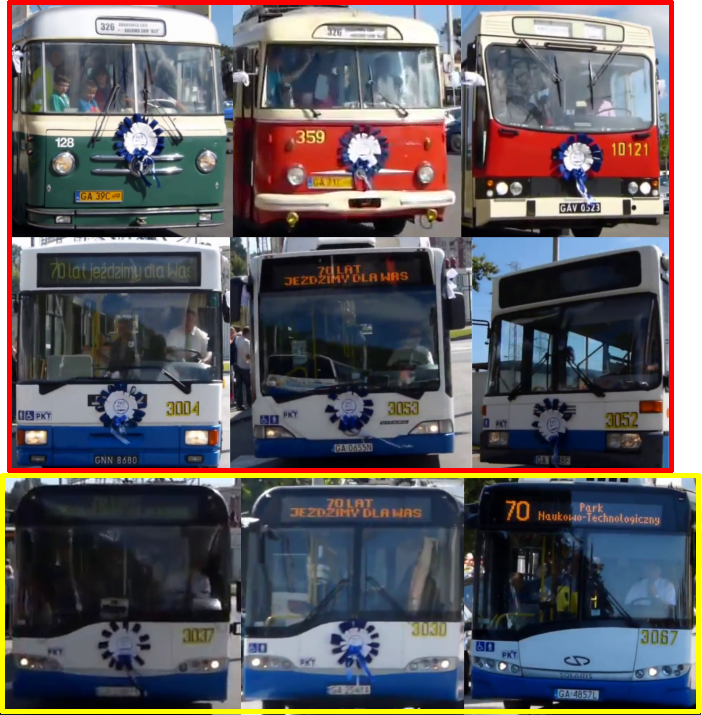
\includegraphics[width=0.8\textwidth]{img/exp_trainig_data_IHa}
    \caption{Typy autobusów zawarte w zbiorze IHarVPkXwSg}
    \label{fig:IHarVPkXwSg_types}
\end{figure}

\begin{table}[!h]
    \centering
    \begin{tabular}{c|c|c}
        Front   & Solaris   & Background \\
        342     & 172       & 1510
    \end{tabular}
    \caption{Liczebność zbioru IHarVPkXwSg}
    \label{tab:IHarVPkXwSg_count}
\end{table}

\newpage

\subsubsection{Zbiór BJZLDmYMFvo}

Zbiór zawiera jedynie dwa modele autobusu Man, jednego
Jelcza i Solarisa. Jedyna uwaga może tyczyć trudności w~odczytywaniu
numeru z~autobusu man/jelcz z~wyświetlaczem w~kolorze zielonym. O~ile
warunki oświetleniowe są dobre - jak na rysunku \ref{fig:BJZLDmYMFvo_types}
- widoczność, a~co za tym idzie rozpoznawalność numeru powinna być na 
zadowalającym poziomie.

\begin{figure}[!h]
    \centering
    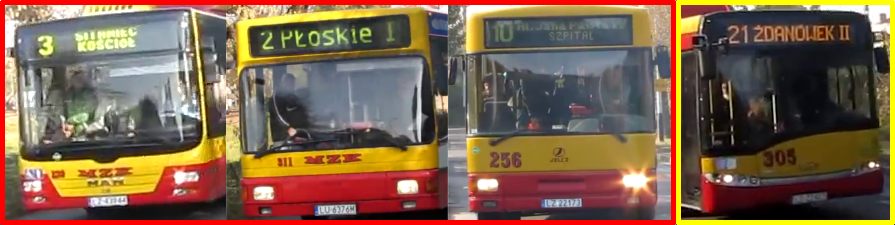
\includegraphics[width=0.95\textwidth]{img/exp_trainig_data_BJZ}
    \caption{Typy autobusów zawarte w zbiorze BJZLDmYMFvo}
    \label{fig:BJZLDmYMFvo_types}
\end{figure}

Zbiór ten posiada drugą co do wielkości 
liczbę obrazów tła. 

\begin{table}[!h]
    \centering
    \begin{tabular}{c|c|c}
        Front   & Solaris   & Background \\
        373     & 8         & 2356
    \end{tabular}
    \caption{Liczebność zbioru BJZLDmYMFvo}
    \label{tab:BJZLDmYMFvo_count}
\end{table}

\subsubsection{Zbiór \_43HUVkrA7E}

Zbiór składający się głównie ze zdjęć zawierających oznaczone fronty
zabytkowego już autobusu Jelcz Berliet. Jeżeli chodzi o~liczebność to 
główną wartością dodaną są borazy reprezentujące tło.

\begin{figure}[!h]
    \centering
    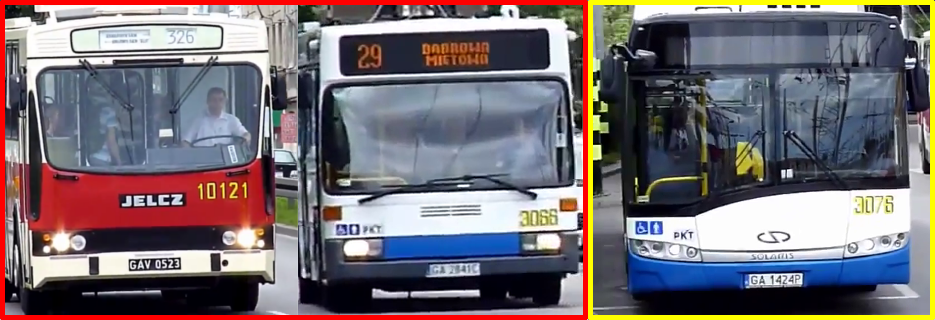
\includegraphics[width=0.75\textwidth]{img/exp_trainig_data__43}
    \caption{Typy autobusów zawarte w zbiorze \_43HUVkrA7E}
    \label{fig:_43HUVkrA7E_types}
\end{figure}

\begin{table}[!h]
    \centering
    \begin{tabular}{c|c|c}
        Front   & Solaris   & Background \\
        44      & 5         & 197 
    \end{tabular}
    \caption{Liczebność zbioru \_43HUVkrA7E}
    \label{tab:_43HUVkrA7E_count}
\end{table}

\subsubsection{Zbiór 8wdvLn40CTk}

Najmniejszy zbiór w~kontekscie różnorodności zawartych modeli. Z~drugiej
strony ogromna ilość obrazów tła i~całkiem sporo oznaczonych ujęć.

\begin{figure}[!h]
    \centering
    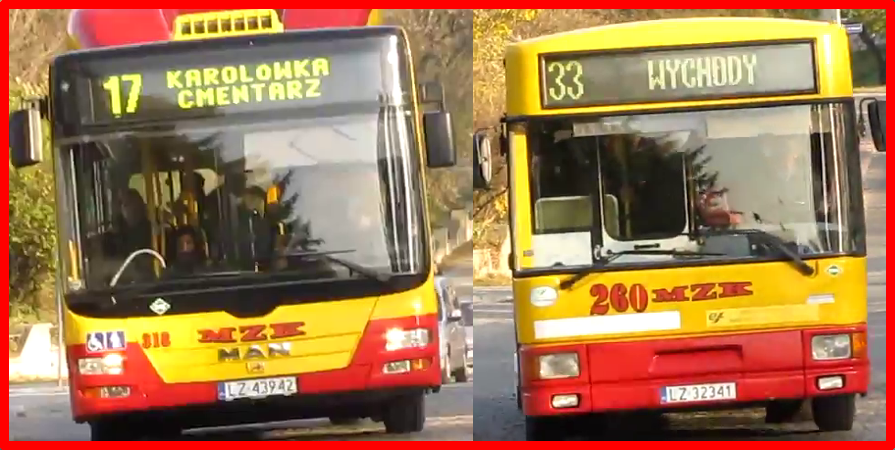
\includegraphics[width=0.45\textwidth]{img/exp_trainig_data_8wd}
    \caption{Typy autobusów zawarte w zbiorze 8wdvLn40CTk}
    \label{fig:8wdvLn40CTk_types}
\end{figure}

\begin{table}[!h]
    \centering
    \begin{tabular}{c|c|c}
        Front   & Solaris   & Background \\
        336     & brak      & 3572
    \end{tabular}
    \caption{Liczebność zbioru 8wdvLn40CTk}
    \label{tab:8wdvLn40CTk_count}
\end{table}

\subsubsection{Zbiór 75Dz6s7S-Tg}

Kolejny niewielki zbiór. Te same modele autobusu Man co w~zestawie
pierwszym. Dodatkowo dwie wersje kolorystyczne (wyświetlacz) modelu
Mercedes Citaro. Na koniec wystąpienie modelu solaris niestety zaledwie
w~dwuch egzęplarzach.

\begin{figure}[!h]
    \centering
    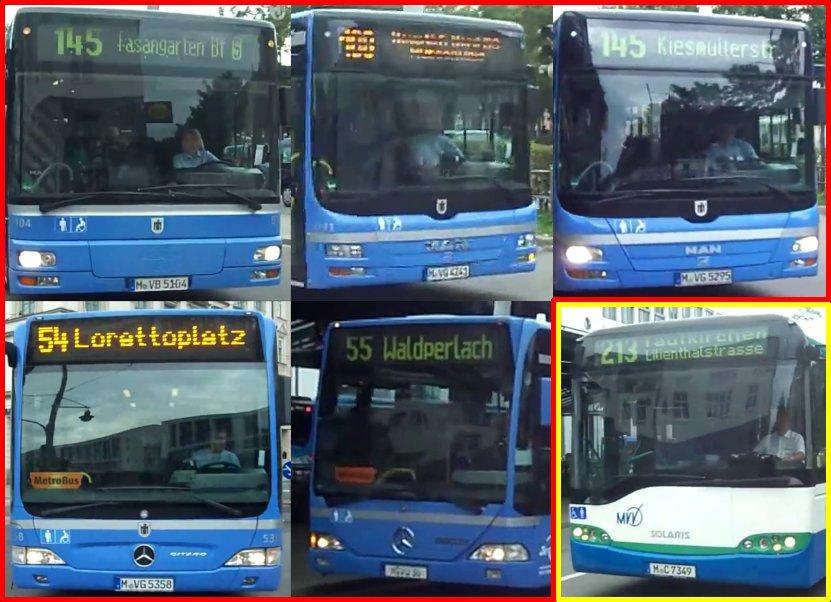
\includegraphics[width=0.75\textwidth]{img/exp_trainig_data_75D}
    \caption{Typy autobusów zawarte w zbiorze 75Dz6s7S-Tg}
    \label{fig:75Dz6s7S-Tg_types}
\end{figure}

\begin{table}[!h]
    \centering
    \begin{tabular}{c|c|c}
        Front   & Solaris   & Background \\
        81      & 2         & 179 
    \end{tabular}
    \caption{Liczebność zbioru 75Dz6s7S-Tg}
    \label{tab:75Dz6s7S-Tg_count}
\end{table}

\newpage

\subsubsection{Zbiór 9hMQ4UGNxhw}

Występujące już wcześniej modele: Mercedes Citaro, zabytkowy Jelcz Berliet,
Man Lion's City, Scania OmniCity, Ikarus 280 z~ledowym wyświetlaczem,
Jelcz M121CNG (x:2, y:1). Dodatkowo dwie wersje kolorystyczne autobusu
Autosan.

\begin{figure}[!h]
    \centering
    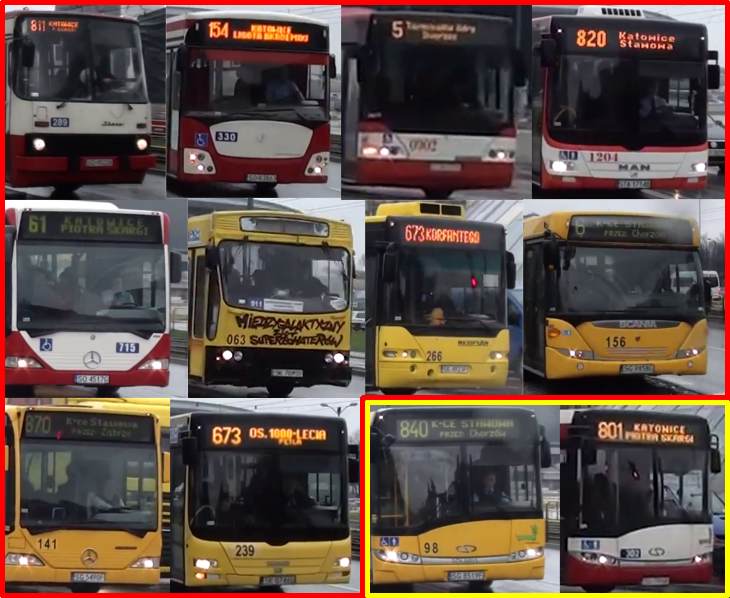
\includegraphics[width=0.95\textwidth]{img/exp_trainig_data_9hM}
    \caption{Typy autobusów zawarte w zbiorze 9hMQ4UGNxhw}
    \label{fig:9hMQ4UGNxhw_types}
\end{figure}

\begin{table}[!h]
    \centering
    \begin{tabular}{c|c|c}
        Front   & Solaris   & Background \\
        267     & 102       & 363 
    \end{tabular}
    \caption{Liczebność zbioru 9hMQ4UGNxhw}
    \label{tab:9hMQ4UGNxhw_count}
\end{table}

Ostatecznie po złączeniu wszystkich zaprezentowanych zbiorów powstały
dwa końcowe (będące jednocześnie punktem wyjścia do dalszych testów):
- zbiór wszystkich oznaczonych frontów (różne + solarisy) - 5781 sztuk,
- zbiór oznaczonych frontów autobusów typu solaris - 955 sztuk.

Osobny zbiór zawierający tylko fronty typu solaris miał na celu
sprawdzenie czy mnogość pozytywnych kształtów nie wpływa na skuteczność
detekcji. Stąd osobne dane uczące/testowe oraz detektor wykrywający 
tylko fronty typu solaris.

\subsection{Przygotowanie optymalnego detektora - eksperymenty}

Pierwsze próby związane z~procesem uczenia detektora miały na celu 
wyłonienie parametrów mających największy wpływ na skuteczność 
oraz efektywność trenowanego detektora.

\subsubsection{Porównanie detektorów HAAR, LBP i HOG}

Pierwsza iteracja uczenia detektorów miała na celu przetestowanie
opcji jakie można zadać narzędziu uczącemu - opencv\_traincascade.

Za zbiór testowy posłużył zestaw oznaczonych zdjęć oraz zdjęć tła
przygotowany dla filmu o id jJ9ixBfVR5k (charakterystyka zbioru
została opisana w~poprzednim rozdziale)

Pierwszy test miał za zadanie wyłonić najefektywniejszą metodę, do dalszych
eksperymentów. Narzędzie dostarczone wraz z~pakietem OpenCV - wspomniany
już opencv\_traincascade - pozwala ,,wyszkolić'' trzy rodzaje
detektorów:

\begin{itemize}
    \item detektor wykorzystujący tzw. cechy Harra - wartość 
        domyślna (HAAR),
    \item detektor LBP,
    \item detektor HOG.
\end{itemize}

Gdy jeszcze nie wszystkie wyłuskane zdjęcia były opisane, wykonany został
krótki test porównaczy skuteczności i~czasu potrzebnego na nauczenie
poszczególnych typów detektorów. Po dość chaotycznie wykonanej próbie
otrzymano następujące wyniki:

\begin{table}[!h]
\centering
\begin{tabular}{r|c|c|c|l}
    & HAAR         & LBP        & HOG              &       \\
    \hline
Solaris & 151  (43\%)  & 81  (23\%) & 61 (17\%)        & /346  \\
Różne   & 1051 (35\%)  & 748 (25\%) & 712 (24\%)       & /2925 \\
Tło     & 635  (11\%)  & 386 (6\%)  & 447 (7\%)        & /5588 \\
\end{tabular}
\caption{Porównanie skuteczności detektorów typu HAAR, LBP i HOG.}
\label{tab:haar_lbp_hog_comparison}
\end{table}

Jako, że nie wszystkie jeszcze próbki były opisane, stąd zaniżona wartość
w~ostatniej kolumnie. Łatwo jednak zaobserwować zgrubny trend dokładności
tychrze detektorów.

O ile czas potrzebny na nauczenie detektora kontra kontra jego skuteczność
dla porównania HAAR kontra LBP był skorelowany i~sensowny. HAAR potrzebował
zdecydowanie więcej czasu na proces trenowania ale za to okazał się
skuteczniejszy. LBP natomiast poświęcił skuteczność na rzecz czsu szkolenia.
To HOG w~tym przypadku dał ciała na obu frontach. Nie dość, że uczył się
dłużej od LBP to jest jeszcez od niego mniej skuteczny.

Czasy uczenia dla poszczególnych detektorów wyglądały następująco:
\begin{itemize}
    \item HAAR - 6 godzin
    \item HOG - 3 godziny
    \item LBP - 40 min
\end{itemize}

\subsubsection{Porównanie detektorów - Solaris kontra reszta zbioru}

Wbrew obawom detektor wyszkolony przy użyciu wszystkich frontów radzi
sobie znacznie lepiej w~wykrywaniu frontów autobusów Solaris niż ten
wyszkolony z~użyciem tylko tego rodzaju frontów. Wyniki dla ustawień
domyślnych dla detektorów typu LBP przedstawiono w tabelce nr 
\ref{tab:sol_vs_all}.

\begin{table}[!h]
    \centering
    \begin{tabular}{r|c|c|l}
            & Solaris(detektor) & Wszystkie typy (detektor) &           \\
            \hline
wszystkie   & 175 (3\%)         & 3466 (71\%)               & 4836      \\
solarisy    & 609 (63\%)        & 854 (89\%)                & 955       \\
błędy       & 289 (1\%)         & 56088 (310\%)             & 18048     \\
    \end{tabular}
    \caption{Skuteczność detektorów wyszkolonych tylko dla typów solaris kontra tych wyszkolonych dla wszystkich typów frontów}
    \label{tab:sol_vs_all}
\end{table}

Jak widać problemem nie jest skuteczność wykrywania istniejących obiektów
tylko ogromna liczba wyników błędnych. W~kolejnych krokach zostaną opisane
próby poradzenia sobie z~tym problemem.

\subsubsection{Parametry minHitRate i~maxFalseAlarmRate}

Niestety wraz ze zwiększaniem parametru minHitRate znacząco zwiększała
się liczba błędnych trafień. Poniższe wykresy przedstawiają znaczny wzrost
błędnych wyników oraz znacznie wolniejszy przyrost odsetka pozytywnych 
rezultatów.
\begin{center}
\begin{tikzpicture}
\begin{axis}[
    title=Błędne trafienia,
    ylabel={$falseAlarmHits$},
    xlabel={$minHitRate$},
    minor y tick num=1,
]
\addplot table {data/hitratio_fal.dat};
\end{axis}
\end{tikzpicture}
\end{center}

Sądząc po poniższym wykresie poziom 80\% jest jak najbardziej do
osiągnięcia. Po dodatkowym zmniejszeniu liczby fałszywych alarmów 
do akceptowalnych wartości (<20\%) detektor w~wersji 0.1 alpha będzie
można uznać za ukończony.

\begin{center}
\begin{tikzpicture}
\begin{axis}[
    title=Pozytywne trafienia,
    ylabel={$posotiveHits$},
    xlabel={$minHitRate$},
    minor y tick num=1,
    legend style={at={(0.06,0.73)},anchor=north west}
]
\addplot table {data/hitratio_fro.dat};
\addlegendentry{wszystkie}
\addplot table {data/hitratio_sol.dat};
\addlegendentry{solaris}
\end{axis}
\end{tikzpicture}
\end{center}

Pierwsza próba zmniejszczenia nieudanych trafień polegała na zmianie 
parametru maxFalseAlarmRate podczas uczenia detektora. Wykonano pięć
sesji uczenia detektora dla wartości: od domyślnej 0.5 do 0.1.

\subsubsection{Podejście drugie - usuniecie zdeformowanych frontów}

Podczas oznaczania frontów autobusów nastąpiła pawnego rodzaju
nadgorliwość. Podczas wyboru klatek do późniejszego oznaczenia
wystąpienia frontu klasyfikowano wszystkie wystąpienia autobusu
czołem do kamery jako poprawne i~wartościowe. Podczas gdy autobus
był ustawiony prostopadle do matrycy aparatu klatka taka była
jak najbardziej poprawna i~zawarte w~niej informacje mogły
z~powodzeniem być wykorzystane podczas uczenia detektora. Jednak
gdy kąt między osią autobusu, a~płaszczyzną matrycy był mniejszy
niż 45 stopni, zdjęcie nie niosło ze sobą informacji przydatnych
w~procesie uczenia. Po pierwsze numer autobusu był już wtedy
niewidoczny - informacja została utracona. Po drugie wprowadzone
zostało zbędne zaburzenie w~wyglądzie szukanych obiektów,
które mogłoby niekorzystnie wpłynąć na skuteczność wyszkolonych
w~ten sposób detektorów.

W~ramach drugiej iteracji poszukiwania optymalnego detektora
usunięto wszystkie oznaczenia frontu posujące do opisu
z~poprzedniego akapitu. Kilka takich przypadków można
zaobserwować na zdjęciu poniżej.

\begin{figure}[h!]
    \centering
    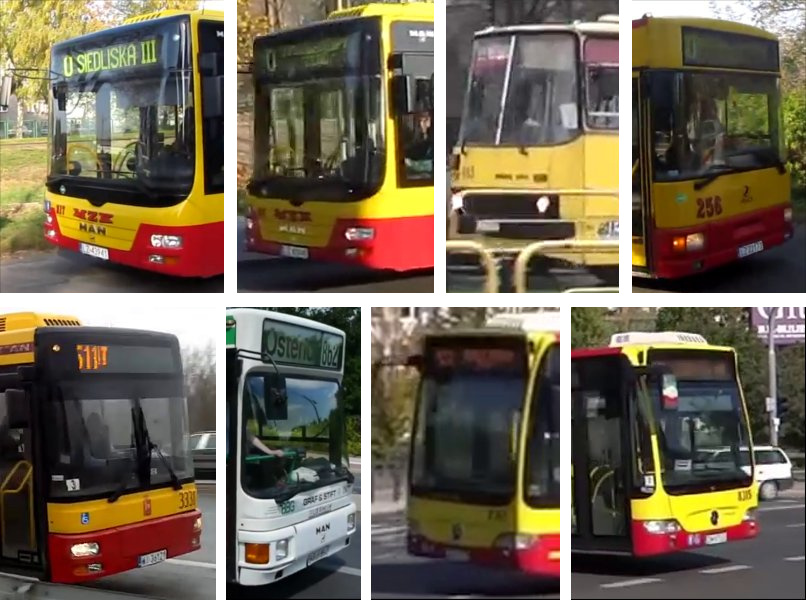
\includegraphics[width=0.8\textwidth]{img/exp_removed_distorted_fronts}
    \caption{Usunięte oznaczenia ze względu na zniekształcenia geometryczne}
\end{figure}

Jednak zanim przejdziemy do weryfikacji skuteczności poprawionego
zbioru, przedstawione zostanie porównanie skuteczności już nauczonych
detektorów. W~poprzednich podrozdziałach (bardzo chaotycznie) opisane
zostały pierwsze próby utworzenia optymalnego detektora. W~ramach
tych eksperymentów powstało 15 plików definiujących detektory, do utworzenia
których użyto zmiennych parametrów. W~pierwszej iteracji zmianie podlegały
parametry:

\begin{itemize}
\item featureType - HAAR(default), LBP, HOG,
\item minHitRate - minimalna procentowa wartość pozytywnych wykryć (domyślnie 0.995),
\item maxFalseAlarmRate - maksymalna procentowa wartość błędów (domyślnie 0.5),
\item numNeg - liczba obrazów tła do wykorzystania.
\end{itemize}

Dodatkowo powstały dwa detektory LBP osobno dla frontów typu solaris i~dla
całości zbioru (5690 wystąpień). Oto cała lista plików z~pierwszej iteracji:

\begin{enumerate}
\item dev\_01\_haar\_default.xml
\item dev\_02\_lbp\_default.xml
\item dev\_03\_hog\_default.xml
\item dev\_04\_lbp\_solaris\_943.xml
\item dev\_05\_lbp\_all\_5690.xml
\item dev\_06\_lbp\_all\_posratio\_996.xml
\item dev\_07\_lbp\_all\_posratio\_997.xml
\item dev\_08\_lbp\_all\_posratio\_998.xml
\item dev\_09\_lbp\_all\_posratio\_999.xml
\item dev\_10\_lbp\_all\_posratio\_999\_maxfalse\_04.xml
\item dev\_11\_lbp\_all\_posratio\_999\_maxfalse\_03.xml
\item dev\_12\_lbp\_all\_posratio\_999\_maxfalse\_02.xml
\item dev\_13\_lbp\_all\_posratio\_999\_maxfalse\_01.xml
\item dev\_14\_lbp\_all\_posratio\_999\_numneg\_2000.xml
\item dev\_15\_lbp\_all\_posratio\_999\_numneg\_4000.xml
\end{enumerate}

Pierwsze trzy pliki utworzone były na ograniczonym podzbiorze danych, gdyż
nie wszystkie próbki były wtedy opisane.

Procedura porównywania skuteczności operowała zbiorze obrazów
reprezentujących wystąpienia frontów autobusów solaris połączonym
z~ogólnym zbiorem ze wszystkimi typami autobusów. Poprawne
wykrycie liczone było wtedy gdy współrzędne prostokątów wykrytego
i~oznaczonego znajdowały się w~odległości nie większej niż 25\% odpowiadającego
wymiaru prostokąta oznaczonego: dla odciętych i~rzędnych odpowiednio szerokość
i~wysokość prostokąta. Do zliczania błędnych wykryć wykorzystano ten sam zbiór.
Ze względu na ograniczenie czasowe zrezygnowano z~wykorzystania zbioru
obrazów tła. Wyniki zaprezentowano na wykresie poniżej.

\begin{center}
\begin{tikzpicture}
\begin{groupplot}[group style={group size=1 by 2},
height=5cm,width=0.8\textwidth,
legend style={at={(0.03,0.93)},anchor=north west}]
\nextgroupplot
\addplot table {data/15_detectors_comparison_positive_percentage.dat};

\addlegendentry{Skutecznosc}

\nextgroupplot
\addplot table {data/15_detectors_comparison_negative_count.dat};
\addlegendentry{Bledne trafienia}
\end{groupplot}
\end{tikzpicture}
\end{center}

Jak widać wyniki w~większości przypadków oscylowały w~granicach 90\%.
W~odróżnieniu od poprzednich testów, te wykonane były na klatkach obrazu
w~oryginalnej rozdzielczości (wysokość 720p. Kolejnym krokiem będzie znalezienie
optymalnego czynnika skalującego. Innymi słowy jak bardzo można zmiejszyć
obraz wejściowy aby utrzymać wyniki na zadowalającym poziomie.
